% Tento soubor nahraďte vlastním souborem s obsahem práce.
%=========================================================================
% Autoři: Michal Bidlo, Bohuslav Křena, Jaroslav Dytrych, Petr Veigend a Adam Herout 2019

% Pro kompilaci po částech (viz projekt.tex), nutno odkomentovat a upravit
%\documentclass[../projekt.tex]{subfiles}
%\begin{document}
%===UVOD====
\chapter{Úvod}
\todo{Dopsat - az na konci}

%===TEORIE====
\chapter{Aspekty vývoje  videoher}
\todo{Dopsat}

\section{Historie herního vývoje}
\todo{Dopsat}

\section{Labyrintové hry}
\todo{Dopsat}

\section{Herní engine}
Herní engine (také game engine) je softwarový framework využívaný pro tvorbu a vývoj (nejen) videoher. Nabízí mnoho nástrojů pro zjednodušení tvůrčího procesu, jako jsou například podpůrné programy, knihovny, a některé poskytují i speciální programovací jazyky vytvořené specificky pro programovaní her v daném engine~\cite{Valencia-Garcia_2016}. V následující části textu jsou popsány a uvedeny některé příklady z nejpopulárnějších herních enginů (viz obrázek~\ref{most_popular_game_engines}).
\begin{figure}[H]
	\centering
	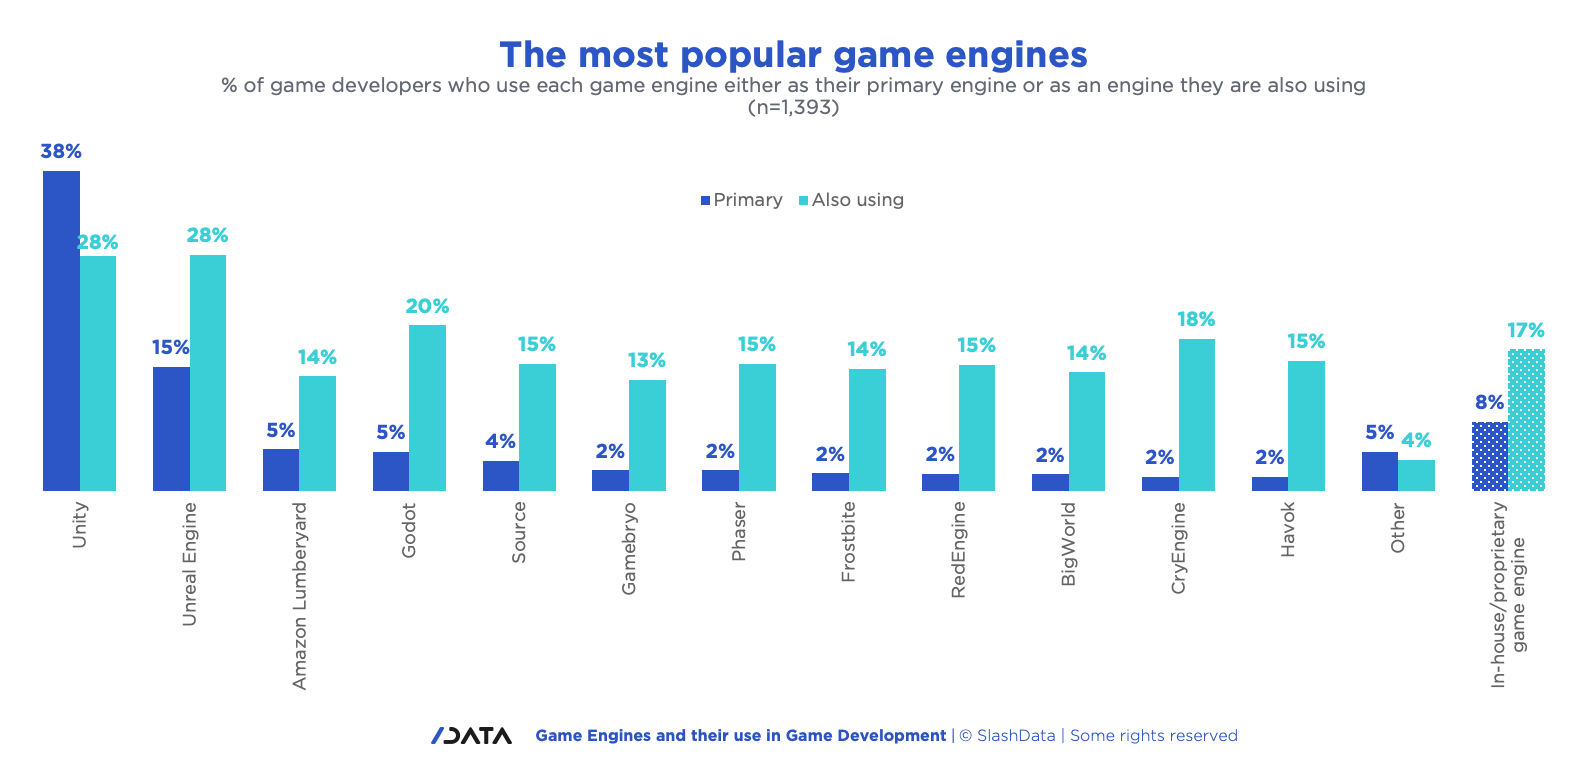
\includegraphics[width=\textwidth]{obrazky-figures/ch2/most_popular_game_engines.png}
	\caption{Výzkum SlashData z roku 2021 o nejpoužívanějších herních enginů. Zdroj~\cite{SlashData_game-engines}}
	\label{most_popular_game_engines}
\end{figure}

\subsection*{Unity}\label{Unity}
Unity je multiplatformní game engine od společnosti Unity Technologies. Dle oficiálních webových stránek aktuálně podporuje více než 20 platforem (např. Windows, macOS, Linux, Android, PlayStation 5, Nintendo Switch~\ldots)~\cite{unity_website}, nejen díky čemuž je jedním z nejpoužívanějších softwarů na tvoření her~\cite{arnia_unity}. Poskytuje bezplatnou verzi (pro soukromé užití, nebo pokud výdělek hry za rok nepřesahuje 100 000\$) i placenou verzi "Unity Pro". 

Pro implementaci her, ať už 2D, 3D či VR (hry pro virtuální realitu), nabízí možnost vizuálního/grafického editoru a skriptů v C\#. Základní herní entita je \verb|GameObject|, které je množné přiřazovat různé vlastnosti, herní mechaniky, grafiku~\ldots a to již předefinované, či naprogramované uživatelem pomocí skriptů. Různé \verb|GameObjects| můžou být součástí \verb|Scene| z čehož je následně konstruován finální produkt~\cite{hocking2015unity}.

Unity je hojně využívána na vývoj AAA (také Triple-A hry, neboli produkt od distributora, pro jehož vývoj byl k dispozici bohatý rozpočet) her, například: Marvel Snap, Apex Legends, ale i indie (takzvaně od nezávislých tvůrců = independent creator), například: Cult of the Lamb, Among Us, Slime Rancher, Cuphead~\cite{unity_case-study}.

\subsection*{Unreal Engine}\label{Unreal Engine}
Unreal Engine je série herních engine, s nejnovější verzí Unreal Engine 5 z roku 2022, od společnosti Epic Games. První verze byla vytvořena pro tvorbu Unreal, 3D střílečky z pohledu první osoby, a byla velmi populární, jelikož díky UnrealScriptu (založeném na C++) mohli uživatele jednoduše původní hru modifikovat~\cite{sanders2016introduction}. Novější verze využívají klasické C++. Podobně jako Unity, nabízí bezplatnou i placenou verzi. Je také multiplatformní, ale podporuje menší škálu platforem než Unity~\ref{Unity} -- základní (Windows, Linux, PlayStation, Nintendo Switch, Xbox), ale podporuje~\cite{Unreal_Engine_FAQ}.

V porovnání s dalšími zástupci herních engine je hodnocen jako jeden ze složitějších~\cite{Kevuru_Games_Unreal-Unity}. Díky své komplikovanější stavbě a strmé křivce učení práce s Unreal Engine je doporučován spíše na větší, komplikovanější projekty, než například na mobilní hry (i přestože podporuje vývoj her na Android)~\cite{cap_porovnani}. Unreal Engine 5 je zaměřený hlavně na 3D vývoj a proto přišel s mnoha funkcemi pro vylepšení vykreslování a práci s trojdimenzionálními objekty - jsou to Nanite (vizuální geometrický systém), Lumen (vylepšená práce se světlem) a MetaSounds (managment audia)~\cite{UnrealEngine5}.

Hrami, které byly vytvořeny za pomocí Unreal Engine je například Minecraft Dungeons, Final Fantasy VII Remake, Fortnite nebo Stray~\cite{unreal_engine-games}.
\begin{figure}[H]
	\centering
	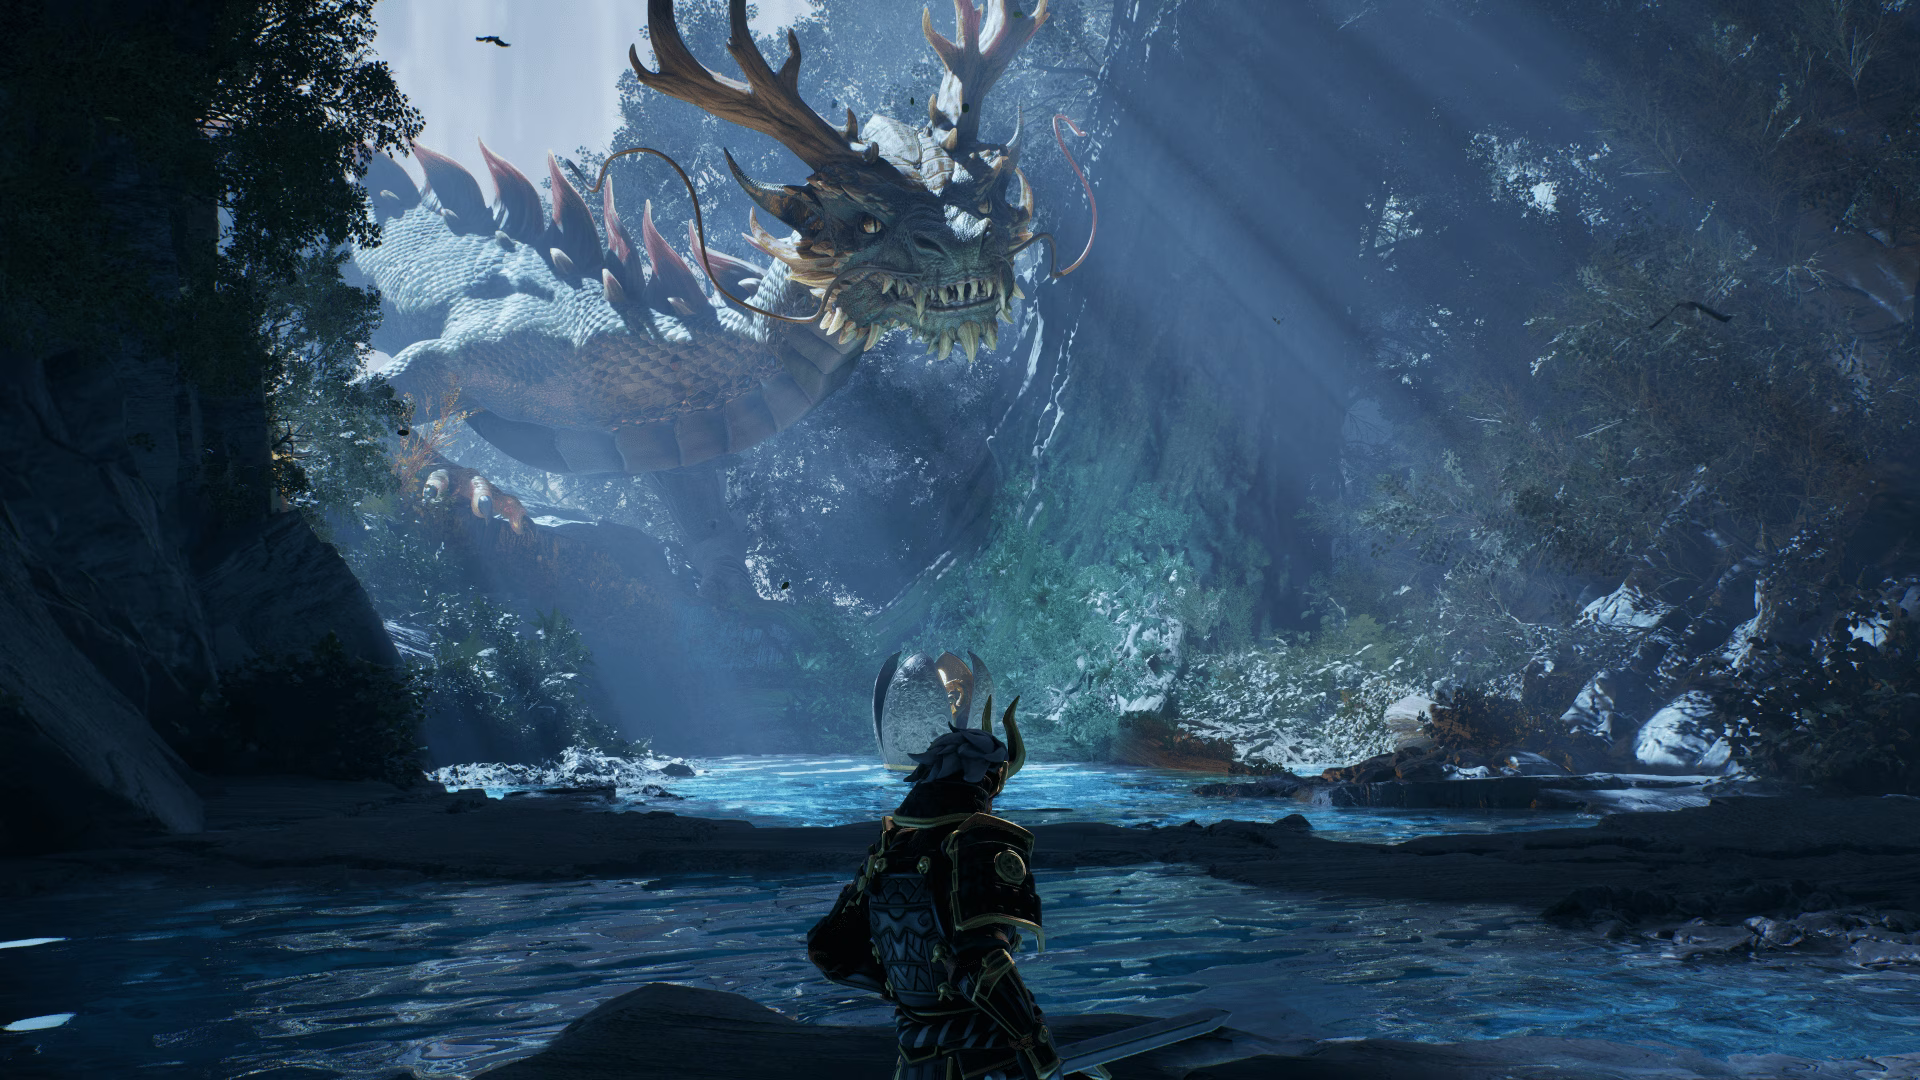
\includegraphics[width=\textwidth]{obrazky-figures/ch2/fortnite.png}
	\caption{Ukázka ze hry Fortnite vytvořená pomocí Unreal Engine 5. Zdroj~\cite{unreal_engine-games}}
	\label{fortnite-unreal_engine}
\end{figure}

\subsection*{Godot}
Godot (s nejnovější verzí 4.2.1) je další software pro tvorbu 3D a 2D her. Na rozdíl od Unity~(\ref{Unity}) a Unreal Engine~(\ref{Unreal Engine}) je od verze 3.0 kompletně zdarma, svobodný a otevřený (open-source)\footnote{\url{https://github.com/godotengine/godot}}. Kvůli tomu má ale Godot oproti jiným zmíněným herním engine omezené oficiální možnosti platforem, jelikož jsou konzole (PlayStation, Xbox) uzavřené ekosystémy a Godot nimi není licencovaný~\cite{Godot_Engine_consoles}. Stále ale podporuje škálu platforem, příkladem desktopové (Windows, Linux, macOS), webové (HTML5), mobilní (Android, iOS) a virtuální realita (Oculus Rift/Quest, HTC Vive).

Základní stavební blok pro vytváření projektu v Godot je \verb|Node| (objekt reprezentující specializovaný prvek) -- tyto objekty lze následně propojovat do \verb|Scene|, což jsou stromy závislostí tvořící finální produkt~\cite{bradfield2018godot}. K těmto \verb|Nodes| lze přiřazovat skripty v jazycích GDScript (dynamicky typovaný jazyk syntaxí podobný Pythonu), C\# a C++\cite{GameEngineWizardry}. Godot se oproti předešlým zmíněným softwarům zaměřuje na 2D, pro které nabízí optimalizovaný přístup zdůrazňující jednoduchost a efektivitu (např. \verb|TileMap|, pro tvoření map, či \verb|Sprite2D| s vlastnostmi pro funkci 2D postav)~\cite{Godot_Engine-features}.

V Godotu byly vytvořeny hry Brotato, Hive Time, Tail Quest a aplikace Dungeoncraft a Material Maker~\cite{Godot_Engine_Showcase}.
\begin{figure}[H]
	\centering
	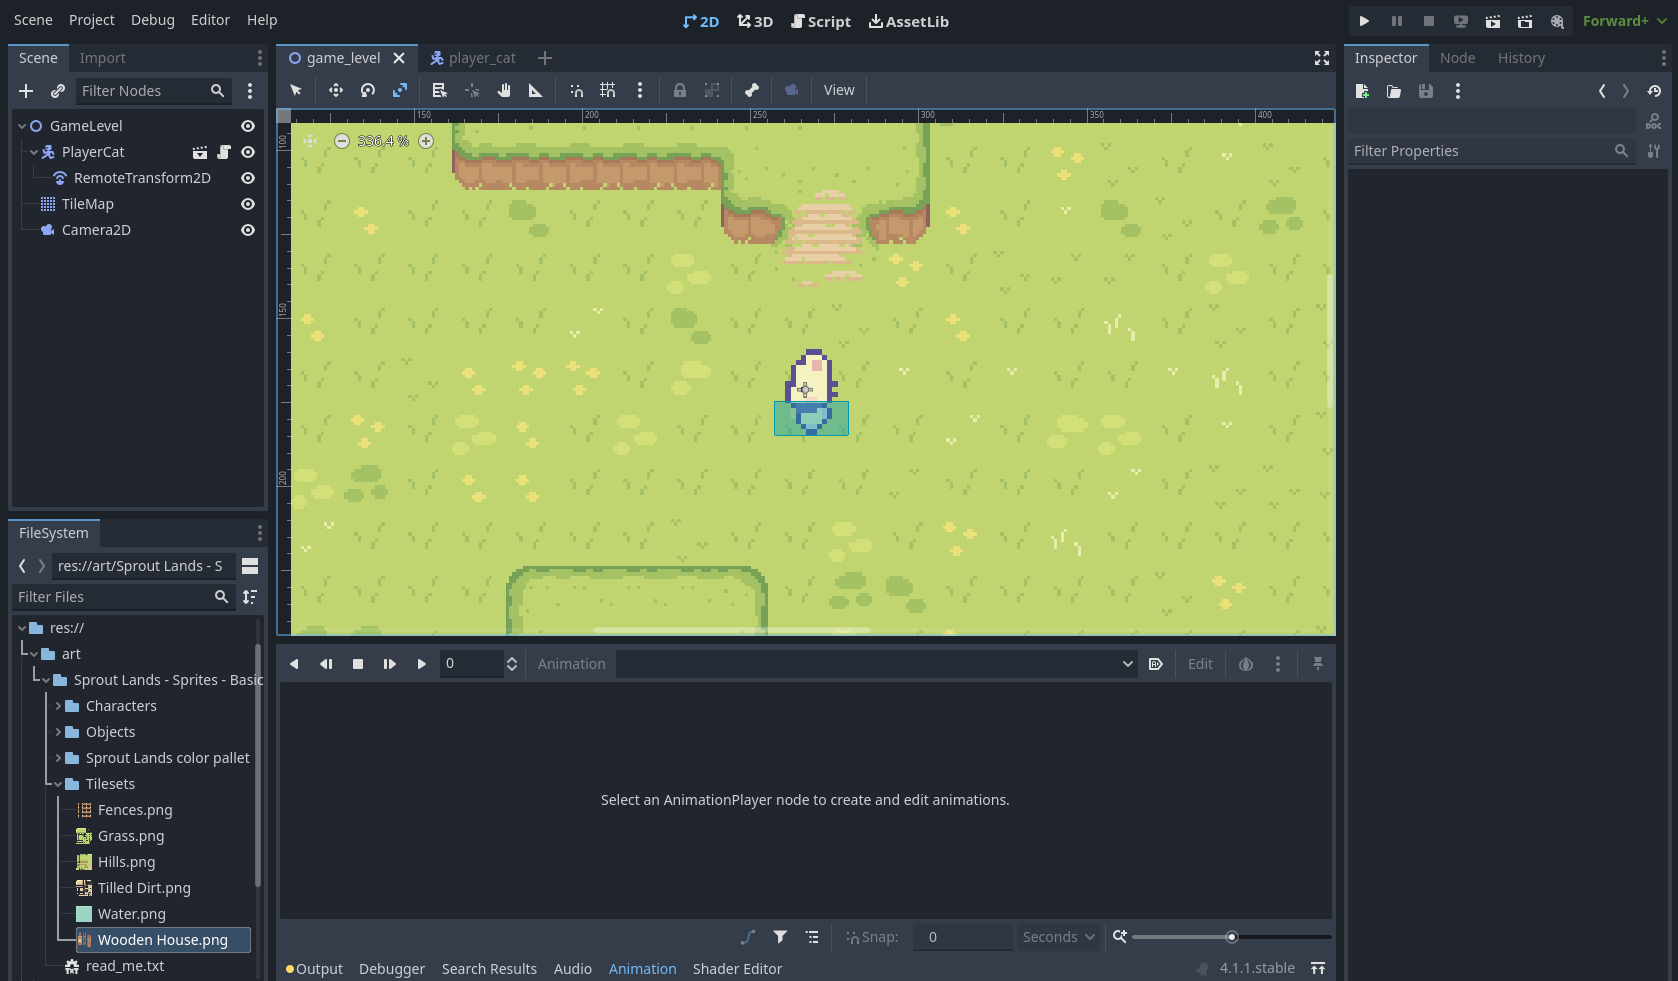
\includegraphics[width=0.8\textwidth]{obrazky-figures/ch2/godot_view.png}
	\caption{Grafické rozhraní Godot verze 4.2.}
	\label{godot_view}
\end{figure}

\section{Celulární automat}
Celulární automat (nadále označován také zkratkou CA) je dynamický systém a diskrétní model prostorového systému využívaný na modelování fyzikálních či biologických simulací. Prostorový systém vyjadřuje prostorovou dekompozici systému - zkoumaný systém je rozdělen na malé části s definovaných chováním~\cite{ims}.

\subsection*{Základní definice }
Celulární automat je čtveřice ${(\alpha^{n}, S, N, f)}$, kterou lze dle Stanfordské encyklopedie filozofie~\cite{sep-cellular-automata}, definovat následovně:
\begin{itemize}
    \item ${ \alpha^{n} }$ (\textit{Lattice}) je diskrétní n-dimenzionální mřížka buněk (${ n >= 1 }$) -- tyto buňky jsou identické (některé mohou být speciální -- např. modelují pevné hranice), 
    \item ${ S }$ je konečná množina stavů, které mohou buňky nabývat -- v každém diskrétním časovém kroku může každá buňka nabýt pouze a jenom 1 stavu, 
    \item ${ N }$ je konečná množina sousedících buněk (okolí, které může, či nemusí obsahovat i buňku samotnou) pro každou buňku, na kterém záleží její vývoj, ${ N \subseteq \alpha }$,
    \item ${ f }$ je konečná množina pravidel pro přechod mezi stavy -- v každém časovém kroku každá buňka aktualizuje svůj aktuální stav podle deterministické přechodové funkce $\phi : \Sigma^n \rightarrow \Sigma$, která mapuje okolí. Často (i když ne nutně) se počítá, že aktualizace synchronní a bere jako vstup okolí v čase $t$ sousední stavy v bezprostředně předchozím časovém kroku $t-1$.
\end{itemize}
CA Game of Life \todo{ref} tedy lze zapsat jako:
\begin{equation*}
\begin{split}
    & \left( \alpha^{2}, \right. \\
    & \left. \{0, 1\}, \right. \\
    & \left. N(c_i) = \{ c_{i-1,j-1}, c_{i-1,j}, c_{i-1,j+1}, c_{i,j-1}, c_{i,j}, c_{i,j+1}, c_{i+1,j-1}, c_{i+1,j}, c_{i+1,j+1} \}, \right. \\
    & \left. \{B3/S23\} \right)
\end{split}
\end{equation*}

Vlastnosti CA můžeme popsat také pomocí řetězců pravidel (anglicky \textit{rulestring}). V následujícím textu jsou uvedeny 2 příklady přebrané ze stránky LifeWiki~\cite{LifeWiki} pro 2 stavové CA. Těmito stavy jsou 1 = živá buňka a 0 = mrtvá buňka. 
\begin{itemize}
    \item \textit{Birth/Survival} notace -- Nejpoužívanější notace, která je zapisována pomocí \verb|B{list}| \verb|/S{nlist}|. Notace je vyjadřována 2 seznamy. V prvním (B) je zapsán počet živých sousedů potřebný pro vznik nové živé buňky, neboli oživení. Druhý seznam určuje kolik živých sousedů musí buňka mít, aby přežila do dalšího kroku. Game of Life by touto notací byla zapsána B3/S23.
    \item S/B notace -- Dříve často používaná, dnes spíše nahrazena Birth/Survival notací. Podobně jako ona je zapisována pomocí 2 seznamů \verb|{list}|\verb|/{list}|. Jeden označuje počet živých sousedů potřebných pro přežití živé buňky a druhý počet živých sousedů potřebných pro oživení mrtvé buňky. Tedy opak Birth/Survival listu. Game of Life je zapsána jako 23/3.
\end{itemize}

Typ okolí závisí na tvaru buněk (čtverec, hexagon \ldots) a také typu prostoru (1D, 2D \ldots)~\cite{ims}. Dvě nejpoužívanější okolí jsou Moorovo a Von Neumannovo s různými variacemi (viz obrázek xxx)~\cite{sloot2004cellular}. Ukázky okolí:
\begin{figure}[h]
    \centering
    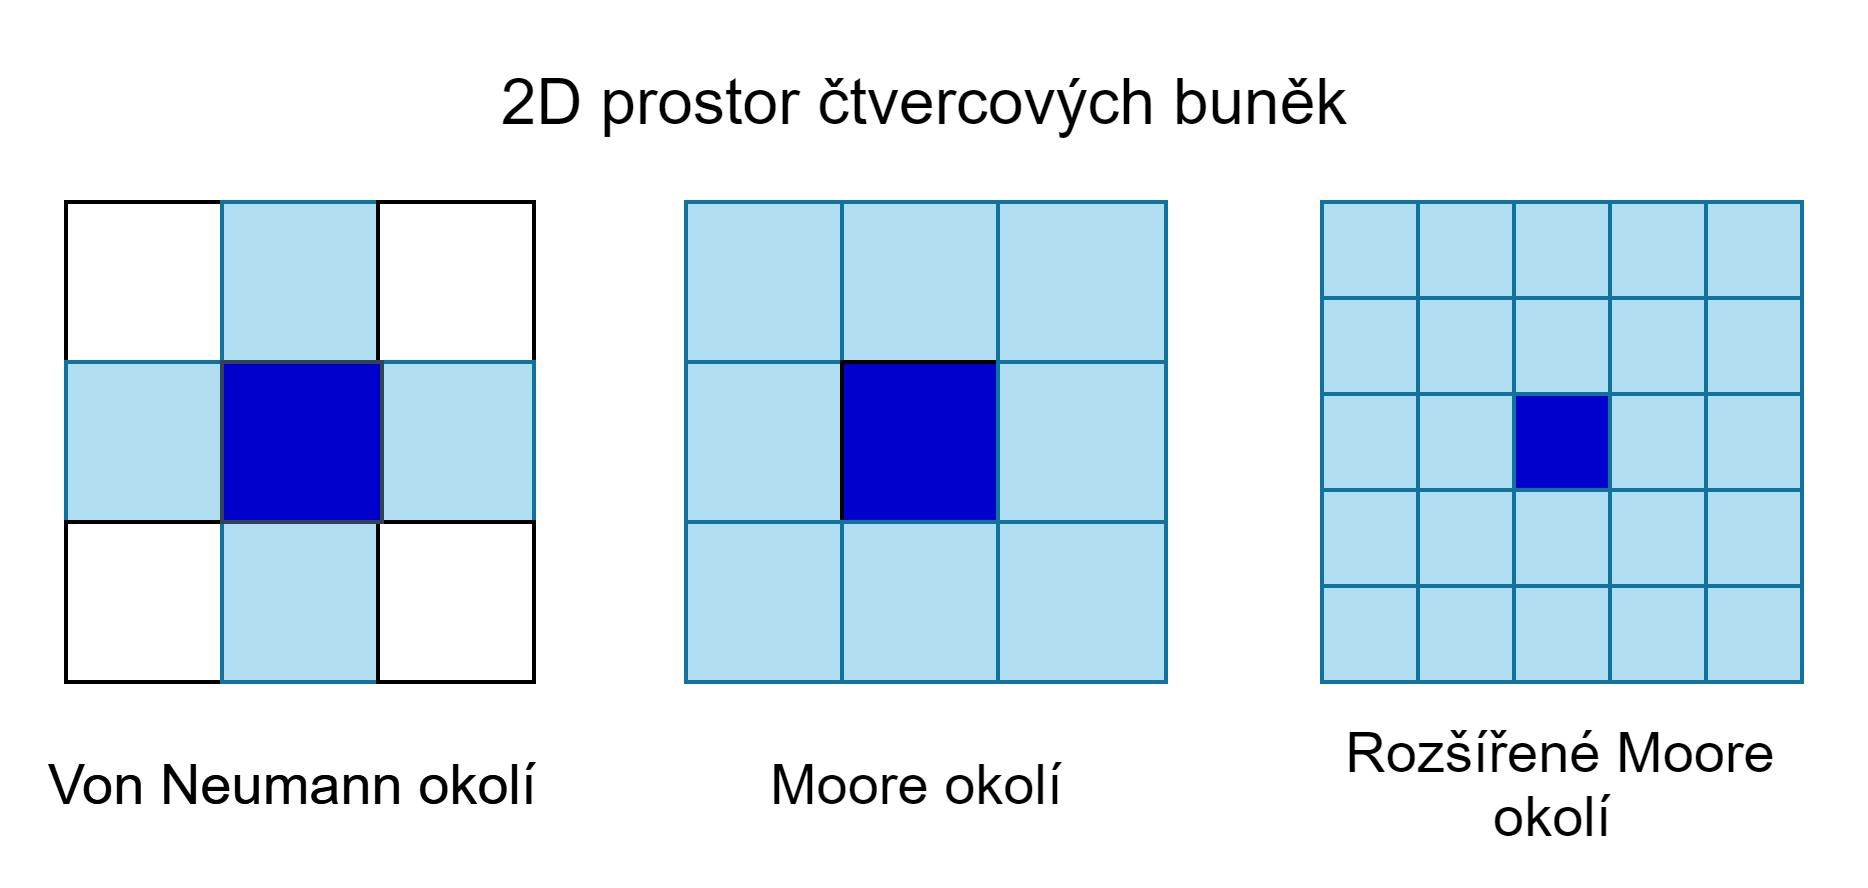
\includegraphics[width=0.48\textwidth]{obrazky-figures/ch2/2D-okoli.png}\hspace{0.5cm}
    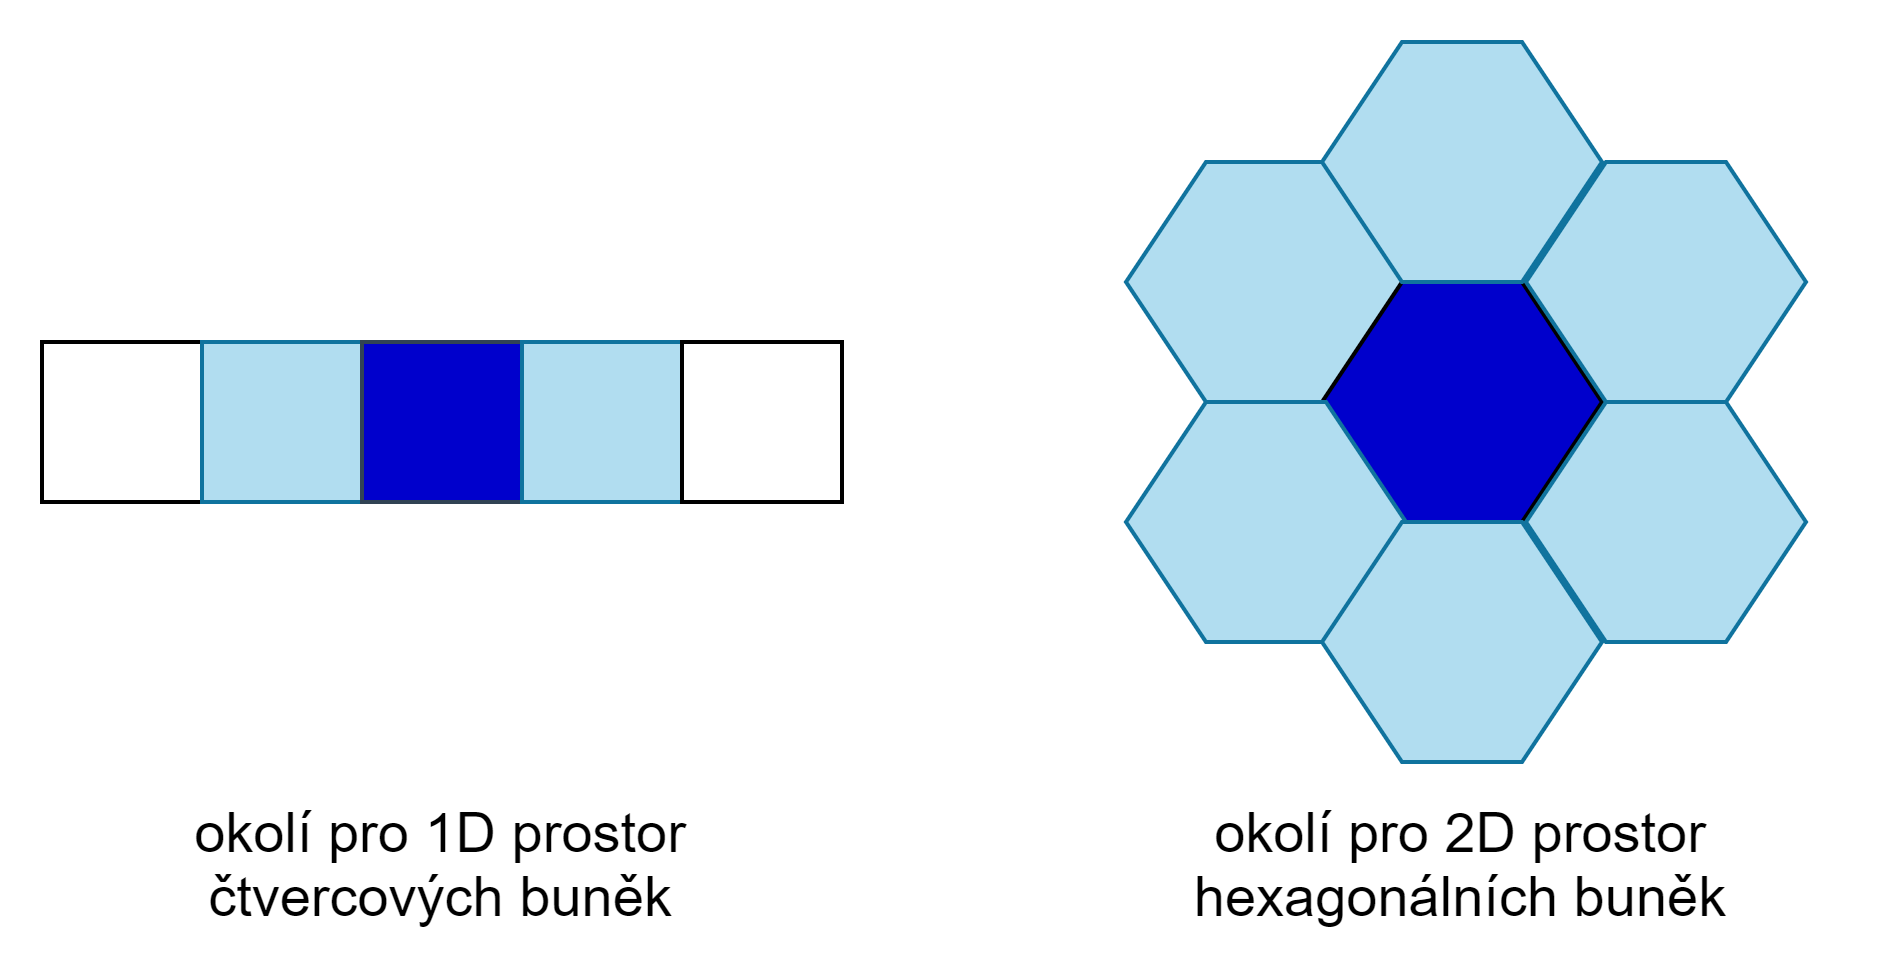
\includegraphics[width=0.47\textwidth]{obrazky-figures/ch2/jina-okoli.png}
    \caption{Příklady okolí (tmavě modrá = zkoumaná buňka, světle modrá = okolí)}
    \label{2D-okoli}
\end{figure}

Jak je již popsáno u formálního popisu, pravidla určují následující stav buňky v čase, který je závislý pouze na jejím aktuálním stavu a stavu jejího okolí a to pro všechny možnosti vstupu. Každé pravidlo je zapsáno jako funkce stavu buňky ${s(t)}$ a jejího okolí ${N_s(t)}$:
\begin{equation*}
s(t + 1) = f(s(t), N_s(t)) \tag*{Zdroj \cite{ims}}
\end{equation*}

Některá pravidla mohou mít i vlastnosti udávající typ pravidlu, které definuje~\cite{mechanics-CA}:
\begin{itemize}
    \item \textbf{totalistic} = o výsledku rozhoduje součet hodnot vstupních buněk (např. Game of Life),
    \item \textbf{legal} = z nulového vstupu nemůže samostatně vzniknout nenulový.
\end{itemize}

\subsection*{Klasifikace}
Stephen Wolfram ve své knize \textit{A New Kind of Science}~\cite{wolfram-NewKindOfScience} definoval 4 třídy pro dělní CA, kterými jsou:
\begin{enumerate}
    \item Téměř všechny počáteční vzory CA se po konečném počtu kroků dostanou do 1 stabilního, homogenního stavu. Zmizí jakákoliv náhodnost v počátečním vzoru.
    \item Téměř všechny počáteční vzory CA se vyvinou do periodicky se opakujících (oscilujících) struktur/stavů nebo zůstane stabilně v některém ze stavů.
    \item Deterministický chaos - téměř všechny počáteční vzory se vyvíjejí pseudonáhodným, nebo chaotických způsobem. Stabilní struktury, které se objeví jsou rychle zničeny okolním hlukem.
    \item Téměř všechny počáteční vzory se vyvíjejí do struktur, které interagují složitým a zajímavým způsobem, s tvorbou místních struktur, které jsou schopny přežít po dlouhou dobu. Konečným výsledkem mohou být stabilní nebo oscilující struktury typu 2 (k dosažení může být ale potřeba velký počet kroků). Pod tuto třídu patří Game of Life.
\end{enumerate}

Některé celulární automaty můžeme označovat také jako \textbf{reverzibilní}. V opoře předmětu IMS~\cite{ims} jsou definované jako systémy, které neztrácí informaci při svém vývoji v čase - což znamená, že v každém okamžiku lze otočit vývoj času a navrátit se k předchozím stavům. Reverzibilní nejsou nikdy CA 4. třídy~\cite{ims}.

\subsection*{Historie - Game of Life}
\todo{Game of Life}

\subsection*{Využití celulárních automatů ve hrách}
Jedním z využití CA obsahují hry "padajícího písku", neboli \textit{Falling-sand games/simulators}. Tyto hry jsou nejčastěji 2D, sandboxové (= podporující kreativitu), jsou založeny například na blokovému/rozdělujícímu celulárnímu automatu, které mohou simulovat reálnou fyziku, jelikož jsou reverzibilní a dodržují fyzikální zákon zachování hmot~\cite{schiff2011cellular}. Nejjednodušší okolí využívané na vyhodnocení těchto CA je Margolusovo (viz obrázek \ref{fig:Margolus}) -- 2D mřížka je rozdělena na 2x2 čtverce, které se každou generaci posouvají diagonálně o jednu buňku~\cite{schiff2011cellular} (okolí v čase t se tedy skládá ze všech buněk, které se nacházejí v bloku v aktuálním čase).
\begin{figure}[h]
    \centering
    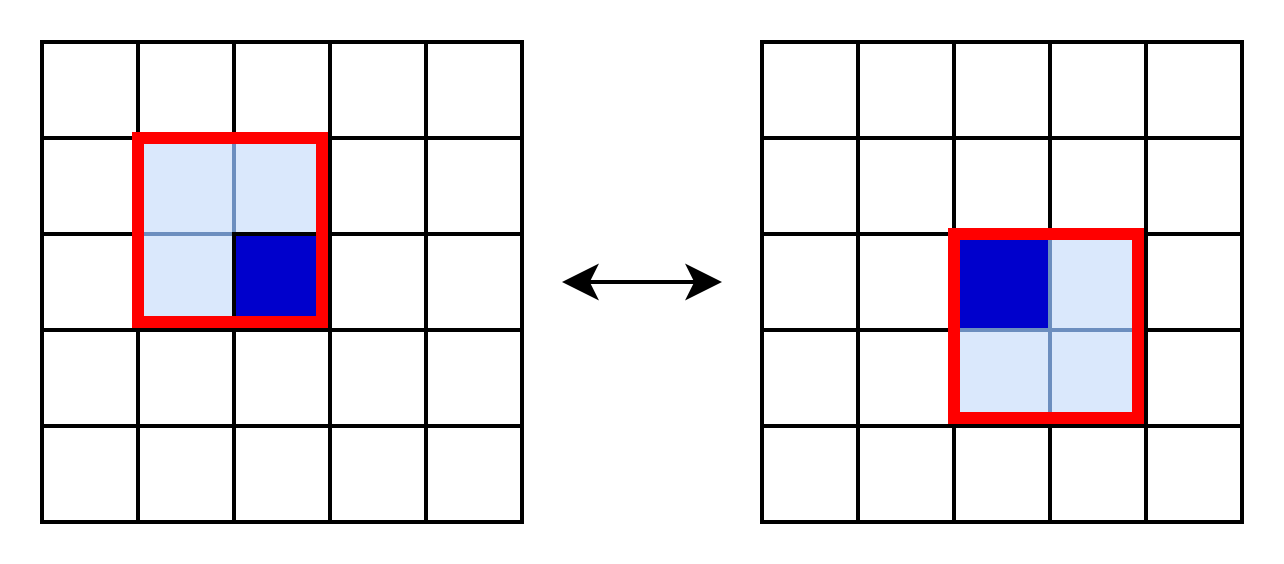
\includegraphics[width=0.48\textwidth]{obrazky-figures/ch2/Margolus.png}
    \caption{Margolusovo okolí (tmavě modrá = zkoumaná buňka, červená = 2x2 blok, světle modrá = okolí)}
    \label{fig:Margolus}
\end{figure}

\noindent Hráč má při hraní hry přístup k několika materiálům/elementům, které mají každý své vlastní vlastnosti (gravitace, reaktivnost s jinými materiály), se kterými může interagovat na dané ploše. Příkladem těchto her může být The Powder Toy~\footnote{https://powdertoy.co.uk}, The Sandbox (2012), Sandspiel či Noita (hra doplněná o roguelike aspekt).
\begin{figure}[h]
    \centering
    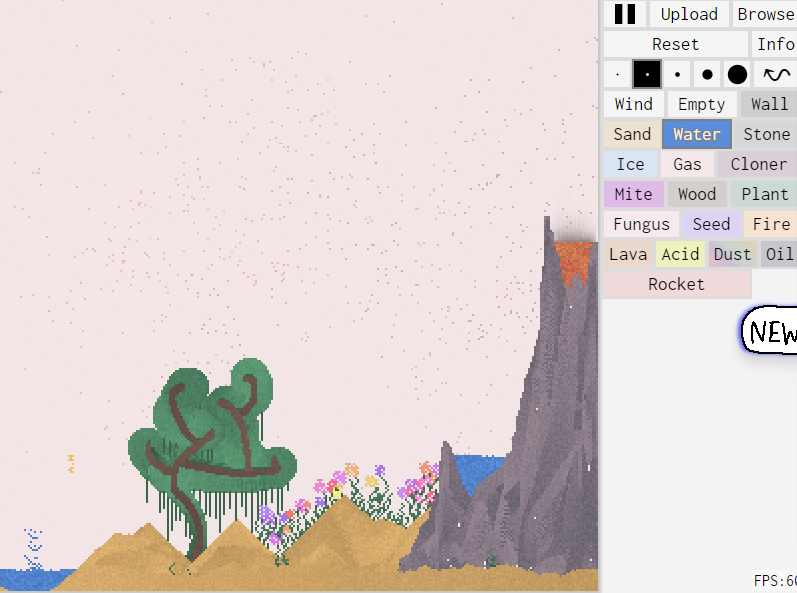
\includegraphics[width=0.6\textwidth]{obrazky-figures/ch2/SandSpiel.png}
    \caption{Ukázka ze hry Sandspiel}
    \label{fig:Sandspiel}
\end{figure}
\newline

Rozšířenější, a v moderních hrách i častější, je využití CA na procedurální generování terénu -- to můžeme najít ve hrách jako je Terraria, Minecraft  či No Man’s Sky~\cite{Procedural_Game_Map}. Tento přístup nalezneme u her vyžadujících větší a pestrý svět, či vysoký počet úrovní vyžadujících rozmanité překážky. Je to jelikož klasické "lidský" výtvory mohou být drahé 2 způsoby. Manuální navrhovaní obrovské mapy, či 100+ úrovní lidmi zabere mnoho času, energie a může naskytnout repetitivita, také tyto před-vytvořené mapy zabírají mnoho paměti a jejich načítaní může být obtížné na procesor -- procedurální generace tedy vytváří mapy za chodu aplikace, takže vyřeší oba problémy~\cite{Procedural_Game_Map}.

Minecraft například generuje základ své mapy díky stochastickým celulárním automatům spuštěných nad zpracovanými(např. pomocí šumu) výsledky kongruenciálních generátorů~\cite{Minecraft}. Stochaistické/Náhodné celulární automaty, jsou CA u nichž nejsou pravidla deterministická (tj. nepředvídatelná), ale pravděpodobnostní -- to znamená, že místo pevného pravidla určujícího následující stav buňky má zadané pravděpodobnosti možných nových stavů buňky~\cite{DBLP:journals/corr/abs-1304-7185}. Díky tomuto dochází k definování přechodů a prolínání mezi různými poddruhy biomů -- například teplé oblasti mají 50\% šanci, že se promění v poušť, 33\% v savanu a 17\% v roviny, nebo oceány mající 50\% šanci, že se promění v zem~\cite{Minecraft}.
\begin{figure}[h]
    \centering
    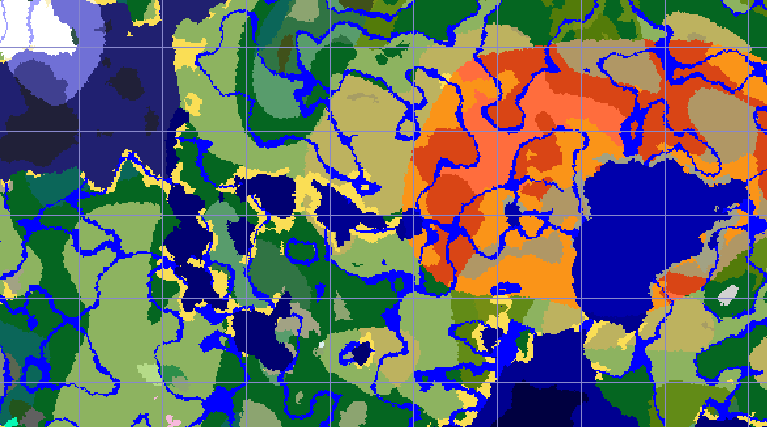
\includegraphics[width=0.6\textwidth]{obrazky-figures/ch2/minecraft_biom.png}
    \caption{Příklad vygenerovaného Minecaft světa s různými biomy}
    \label{fig:minecraft_biom}
\end{figure}
\newline

Některé z jednodušších možností generování prostředí s celulárními automaty je využití algoritmů na náhodné generování jeskyní. Příkladem může být například algoritmus z naučné stránky envatotuts+~\cite{CaveCA}, kde buňka CA může nabýtvat 2 stavů -- živá, mrtvá:
\begin{algorithm}
\caption{Cave Generation Algorithm}\label{cave_gen}
\begin{algorithmic}[1]
\Function{CaveGeneration}{$\text{matrix}, \text{row}, \text{col}$}
    \State $\text{deathLimit}$
    \State $\text{birthLimit}$
    \State $\text{neighbors} \gets \text{countAliveNeighbours}$
    \State $\text{cellValue} \gets \text{matrix[row][col]}$
    \If{$\text{cellValue} = \text{alive}$}
        \If{$\text{neighbors} < \text{deathLimit}$} \Comment{Too many neighbours} 
            \State \textbf{return} $\text{dead}$
        \Else
            \State \textbf{return} $\text{alive}$
        \EndIf
    \Else
        \If{$\text{neighbors} > \text{birthLimit}$} \Comment{Reborn} 
            \State \textbf{return} $\text{alive}$
        \Else
            \State \textbf{return} $\text{dead}$
        \EndIf
    \EndIf
\EndFunction
\end{algorithmic}
\end{algorithm}
\newline
Algoritmus funguje na několika jednoduchých principech, se kterými se dá různě manipulovat a to změnou hodnot \verb|deathLimit| a \verb|birthLimit|:
\begin{itemize}
    \item narození = pokud je buňka mrtvá a má určitý počet živých sousedů, v následující iteraci oživí (podpora růstu jeskynních chodeb)
    \item smrt = pokud je buňka živá a má příliš málo mrtvých sousedů, zemře v následující iteraci (vytváření otevřených prostorů v jeskyni).
    \item přežití = pokud je buňka živá a má dostatečný počet živých sousedů, přežívá do následující iterace (udržování existující struktury jeskyní)
\end{itemize}
\begin{figure}[h]
    \centering
    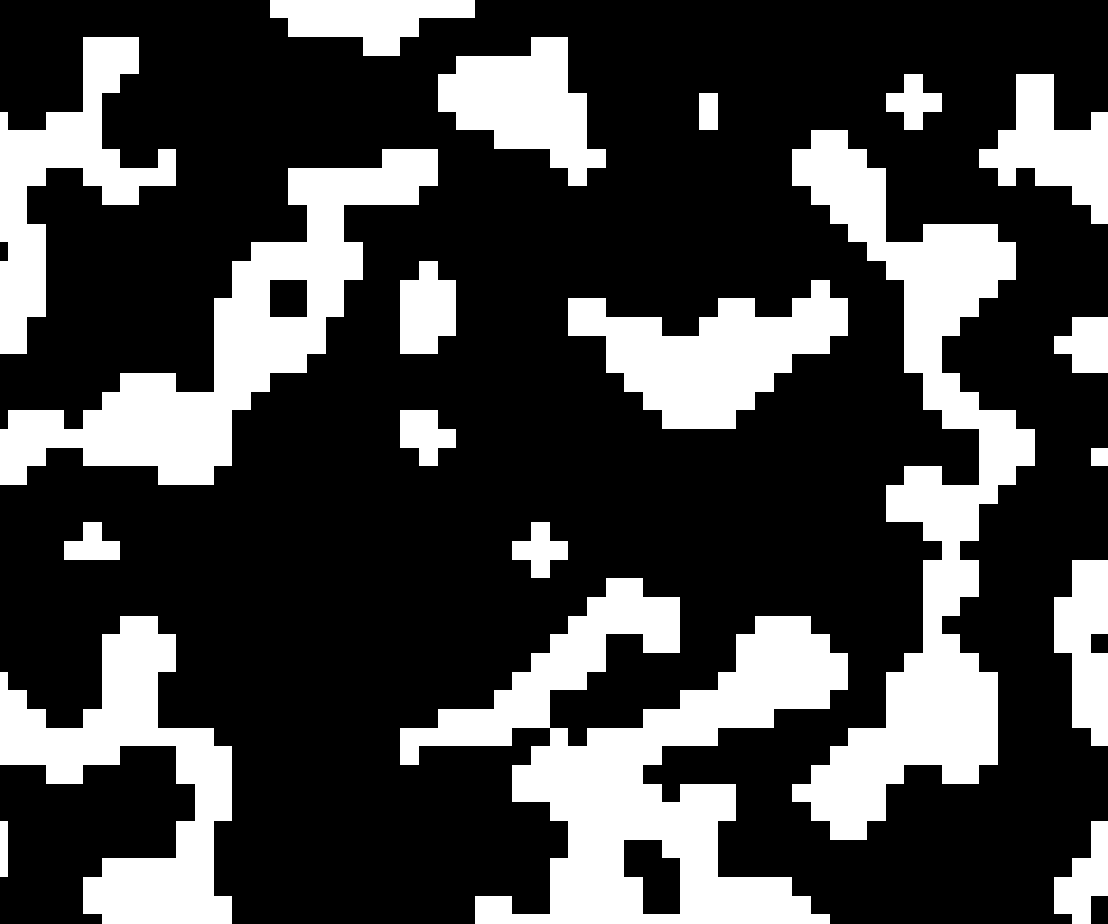
\includegraphics[width=0.3\textwidth]{obrazky-figures/ch2/cave.png}
    \caption{Příklad algoritmu generování jeskyní s využitím Moorova okolí,	deathLimit = 3, birthLimit = 4}
    \label{fig:cave}
\end{figure}

Také je možné využít algoritmy, generující strukturu podobnou bludišti. Celulárními automaty s touto vlastní je OCA:Maze~\cite{OCA:Maze}. Hlavním principem tohoto algoritmu s Mooreovým okolím je, že pokud má buňka živých 1 až 5 sousedů tak přežije a ožívá pokud má přesně 3 sousedy -- to znamená, že je pro buňky složitější zemřít a tím se vytváří vzory podobné bludišti, které ale nejsou zcela propojéné (získáváme mnoho nepropojených místností). Existuje i jeho upravená verze(Mazectric), která ale omezuje počet sousedů potřebný přežití na 1 až 4, díky čemuž vznikají rovnější a delší "cesty"~\cite{OCA:Maze}.
\begin{figure}[h]
    \centering
    
\includegraphics[width=0.40\textwidth]{obrazky-figures/ch2/OCA:Maze.png}\hspace{0.5cm}
    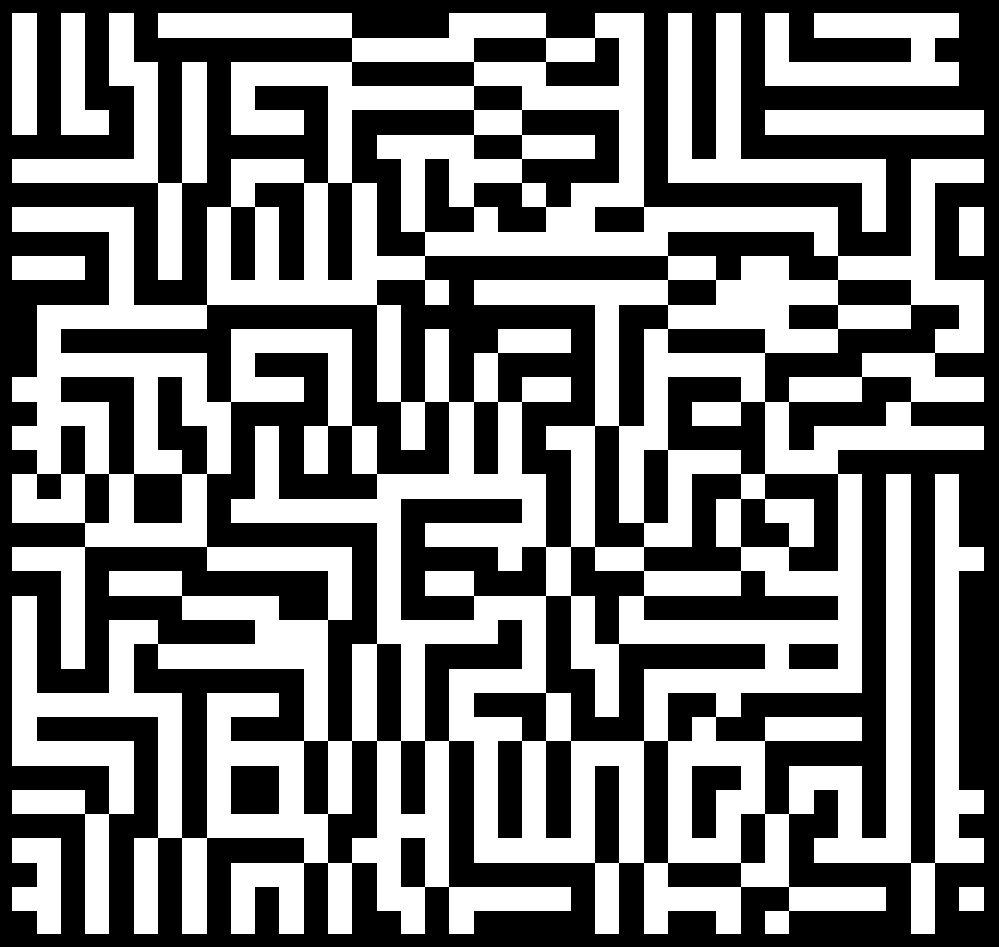
\includegraphics[width=0.40\textwidth]{obrazky-figures/ch2/Mazectric.png}
    \caption{Výsledky CA OCA:Maze a Mazectric}
    \label{2D-okoli}
\end{figure}

\section{Grafové algoritmy}
    \todo{Dopsat - takove to na rozdelení do grup/nalezeni nejkratsi cesty (viz IZU)}
\section{Prohledávání stavového prostoru}
    \todo{Dopsat - BFS~\ldots (z IZU)}

%===KONCEPT====
\chapter{Koncept 2D labyrintové hry}
\todo{Dopsat - popsat koncept typu her obecně (pravidla labyrintových her,..)}

\section{Mechaniky hry}
\todo{Dopsat - kamera, mapa, nepratele, itemy}

\section{Uživatelské rozhraní}
\todo{Dopsat}

%===IMPLEMENTACE====
\chapter{Implementace 2D labyrintové hry} % TODO NECO KONKRETNEJSIHO
\todo{Dopsat}
\section{Generování mapy}
\section{Optimalizace mapy}
\section{Umístění postavy} % start + cil
\section{Experimenty s generováním map pomocí CA} % statistiky, proc jsem vybrala dany postup

%===TESTOVANI====
\chapter{Uživatelské testování}
\todo{Dopsat}
\section{Dotazník}
\section{Analýza výsledků}
\section{Závěr testování}

%===ZAVER====
\chapter{Závěr}
\todo{Dopsat - az na konci}
%===============================================================================

% Pro kompilaci po částech (viz projekt.tex) nutno odkomentovat
%\end{document}
